\Chapter{A virtuális kollaborációs tér}

% A fejezet gyakorlatilag a kliens kialakításáról szól.

% Maga a menü, beállítások és egyéb felületi elemek is lehetnek 3D-sek.

\Section{Megjelenítési mód}

\SubSection {OpenGL, PyOpenGL}

Az OpenGL egy 2D-s és 3D-s vektor grafikus  API, ami elérhető és támogatott a fő operációs rendszereken (Linux, macOS, Windows) valamint számos programozási nyelvvel kompatibilis. \cite{opengl}

Az OpenGL pythonnal használható verziója a cross-platform, nyíltforráskodú PyOpenGL. A PyOpenGL támogatja a GL, GLU és GLUT könyvtárakat. 

Továbbá lehetőség van a PyGame használatára OpenGL-s kódok megvalósításához.

A dolgozathoz tartozó program felhasználja mindhárom könyvtárat és a modell betöltéshez a PyGame-t is.

\SubSection{Modellek}
A program obj kiterjesztésű modellekkel dolgozik, amikhez mtl kiterjesztésű textúrát rendel. 
\begin{itemize}
\item {\bf obj}: A Wavefront Technologies által a Advanced Visualizer animációs csomagjukhoz kifejleszett obj fájlformátum egy geometria-definíciós formátum. 
Annak köszönhetően, hogy ynílt forráskodú más 3D-s grafikus alkalmazások gyártói átvették.

Az obj egy egyszerű formátum ( akár ember által is olvasható), ami semmi mást nem add meg, mint a 3D geometriát. Mint például a csúcsok helyzetét, az egyes textúra koordináta-csúcsok helyzetét, a csúcsok normálisát, az egyes sokszögeket csúcsok listájaként, textúra csúcsokat. \cite{obj}

\item {\bf mtl}: Az MTL fájl egy segédfájl, amely a modell anyagainak meghatározását tartalmazza, amelyekhez OBJ fájl hozzáférhet. Az OBJ fájlnak meg kell adnia az MTL fájl nevét. Az MTL fájl az anyagok definícióinak sorrendjét tartalmazza. Mindegyik definíció egy newmtl utasítással kezdődik, amely meghatározza az anyag nevét, majd azon sorok következnek, amelyek megadják az adott tulajdonságokot.\cite{mtl}
\end{itemize} 

A program fő elemei az ágensek. 
A modell, amit felhasználtam erre a célra egy császárpingvin. 
Minden ágenst egy ilyen modell valósít meg, csupán a színűk változik, ami pedig a programkódban kerül megvalósításba. \\
\begin{figure}[htp]
    \centering
   	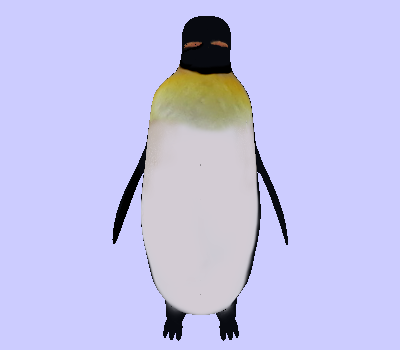
\includegraphics[width=4truecm, height=3truecm]{images/pingvin.png}
	\caption{császárpingvin modell}
\end{figure}

A program szinterének fő eleme a kastély modell, ahol maga a jelenet játszódik.
\begin{figure}[htp]
    \centering
   	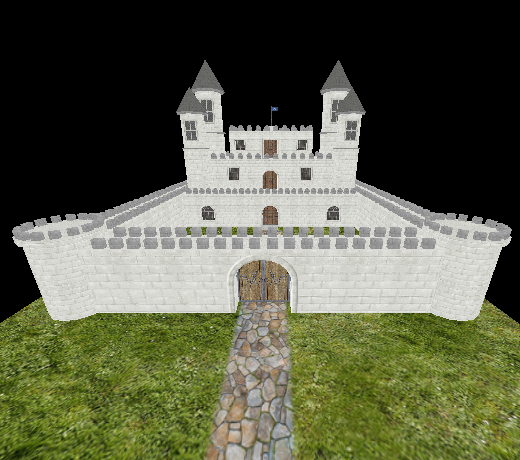
\includegraphics[width=4truecm, height=3truecm]{images/castle.png}
	\caption{kastély modell}
\end{figure}

Felhasználtam továbbá doboz modelleket, amiknek az elmozgatása a feladat. Ezen modellek színének manipulációja szintén a programban történik.
\begin{figure}[htp]
    \centering
   	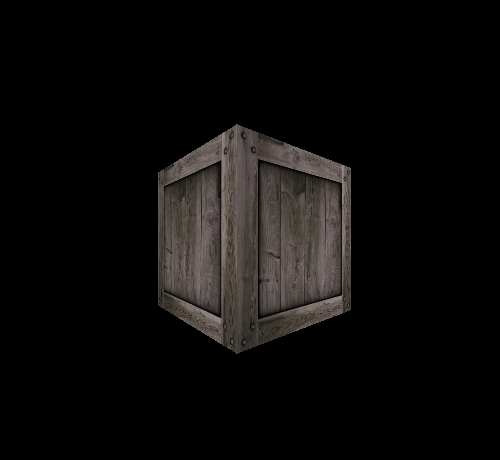
\includegraphics[width=4truecm, height=3truecm]{images/box.png}
	\caption{doboz modell}
\end{figure}

\SubSection{Fények:}

Az objektumok megjelenítéséhez elengedhetetlenek a megfelelő fénybeállítások.\\

„Az ábrázolandó térrészben uralkodó fényviszonyok leírására az alábbi fényösszetevőket szokásfigyelembe venni:

\begin{itemize}
\item A {\bf környezeti fény} (\texttt{ambient light}) az ábrázolandó térrészben mindenütt jelen lévő, állandó intenzitású fény, amelynek forrása, iránya nem ismert (gondoljunk olyan nappali fényre,amikor a nap a felhők mögött van).
\item A {\bf szórt fénynek} (\texttt{diffuse light}) van iránya, mindig valamelyik fényforrásból jön. Fő jellemzője, hogy az objektumokkal ütközve minden irányba azonos módon és mértékben verődik vissza, tehát teljesen mindegy, hogy milyen irányból nézzük az objektumokat, a hatás csak a fényforrástól, az anyagtulajdonságoktól és a pontbeli normálistól függ.
\item A {\bf tükröző fénynek} (\texttt{specular light}) is van iránya és forrása, és hatása nemcsak az anyag-tulajdonságoktól és a pontbeli normálistól, hanem a nézőponttól is függ. Gondoljunk egy sima felületű fémgömbre, amit erős, koncentrált fénnyel világítunk meg. Megfelelő szögből nézve egy fényes (többnyire fehér) foltot látunk, amelynek mérete és helye a nézőponttól függ, fejünket mozgatva a folt is mozog, mígnem eltűnik.”\cite{fenyek_szinek}
\end{itemize}

\SubSection{A modellek átszínezése:}

A modellek átszínezésére az OpenGL \texttt{glColorf} függvényét használtam, ahhoz azonban hogy ezt alkalmazni tudjuk, meg kell érteni, miként értelmezzük a színeket a számítógép grafikában.

,,A színeket legcélszerűbb egy háromdimenziós tér pontjaiként felfogni. A tér egy bázisának(koordináta-rendszerének) rögzítése után minden színt egy számhármas segítségével lehetazonosítani. A számítógépi grafikában két színmegadási (színkeverési) mód, kétféle bázisterjedt el.”
\begin{itemize}
\item  RGB (additív): ,,Additív színkeverés esetén azt írjuk elő, hogy mennyi vörös (Red), zöld (Green) és kék (Blue) színkomponenst adjunk a fekete színhez, a fekete képernyőhöz.”
\item CYM (szubtraktív): ,,Szubtraktív színkeverés esetén azt írjuk elő, hogy mennyi türkiz (Cyan), bíbor (Magenta) és sárga (Yellow) színt kell kivonnunk a legösszetettebb színből, a fehérből (a papírszíne) a kívánt szín előállítása érdekébe.”\cite{fenyek_szinek}
\end{itemize}

A \texttt{glColor} az RGB bázisrendszert használja fel, tehát a három paramétere egy-egy szám, ami a piros, zöld és kék színeket jelöli.

A \texttt{glColor3*}, ahol a * a számok típusát jelöli.(int,float...) Az egész számokra vonatkozó változata a \texttt{glColor3i}), a float \texttt{glColor3f},továbbá a \texttt{glColor4*} rendelkezik egy negyedik paraméterrel is, az \texttt{alpha}-val, ami az átlátszóságot határozza meg.
Például: 
\begin{python}
glColor3f(0.0,0.0,0.0) #fekete
glColor3f(1.0,1.0,1.0) #feher
glColor3f(1.0,0.0,0.0) #piros
glColor3f(0.0,1.0,0.0) #zold
glColor3f(0.0,0.0,1.0) #kek
\end{python}

\Section{Interaktív elemek}

A színtér interkatív elmei az ágensek és a dobozok. 
Az ágensek képesek fordulni, előrehaladni, ugorni. 
A dobozok pedig olyan írányú elmozdulásra, amerre tolják őket.

\SubSection{Animáció}

Ahhoz, hogy a program látványosabb legyen animációkra van szükség, így a modell nem csak elmozul például olyan írányba, amerre szeretnénk, hanem az animáció használata séta hatását kelti.

A modellek formátuma (.obj) azonban nem támogatja az animációkat, ezért minden egyes mozdulatnak külön modell, a hozzátartozó mtl fájllal, készült.

Az animációkat a testvérem készítette el Blender felhasználásával. 

Az animációk elkészítéséhez elsőnek a modell úgynevezett vázára van szükség,azt kell elkészíteni és azt lehet a továbbiakban animálni. 
 
Az elkészült animációk a következők: ugrás, séta és a dobozok tolásához a doboz megfogása és elengedése.
 
A programkódban az animácókat úgy valósítottam meg, hogy egymás után, apró szünetet beiktatva betöltöttem a modelleket egymás helyére.

Fontos, hogy minden egyes mozdulatot rajzolását úgy kell megvalósítani, hogy minden más modell és a kamera képből készült háttér is kirajzolódik.
 
\SubSection{Ütközésvizsgálat}

AZ ágensek megfelelő tértészben tartása végett (tehát ne tudják elhagyni a kastélyt), ne sétáljanak át egymáson, illetve más modelleken, szükség van ütközésvizsgálatra.

Ez azt jelenti, hogy figyeljük a modellek egymáshoz való helyzetét a térben, a távolságot közöttük a \texttt{x,y,z} tengelyeken és ha túl közel kerülnek egymáshoz, akkor megakadályozzuk, hogy tovább haladjon a mozogni képes modell / tovább haladjanak a modellek abba az írányba, ami már nem megengedett.

Ez azt jelenti, hogy  mozoghat  például az \texttt{y} tengelyen, ha az a tiltott, de csak ha \texttt{y} tengelyen felvett értékéhez hozzáadva/kivonva ütközne akadályba, viszont a ellenkező művelettel nem. 

Ha mindkét művelettel akadályba ütközne, akkor nem haladhat az \texttt{y} tengelyen.
 
Az első dolog, amit meghatároztam az az volt, hogy a \texttt{z} tengelyen (ez jelenleg a fel és le írány a játékban) nem sülyedhet 0 alá az ágensek értéke, mert akkor a kastélyba modellbe és alá esne egy részük.

A következő lépésben a tér azon részét határoztam meg, ami a játékteret képezi ( a kastély modell kertje), hogy a falakon ne tudjanak áthaladni a modellek, tehát tényleg ne legyenek képesek elhagyni a játék végéig.

Ez az \texttt{x és y} tengelyre jelent korlátozásokat.

A további lépés az ágensek poziciójának figyelése, hogy az ágensek egymáson se tudjanak áthaladni. Ehhez minden pozició változás előtt meg kell vizsgálni, hogy az adott lépéssel nem kerülnek e a másik modell olyan közvetlen közelébe, ami már nem megengedett.

Mivel a pingvin modellek középpontja a modell közepébe esik, ezért egy bizonyos értéket mindig hozzá kell adni a számításkor ( hogy a modell széleit figyeljük), hogy ne lógjanak egymásba semmilyen esetben sem. 

Az ágenseknél továbbá azt is figyelmbe kell venni, hogy a kódban át lettek méretezve, ezért a poziciójuk koordinátáit is a megfelelő arányban kell növelni/csökkenteni.

Ugyanez vonatkozik a doboz modellek való ütközésvizsgálatra, mindig lesz valamekkora plusz érték, ami a modell szélét hivatott jelenteni.

Az, hogy figyelembe vesszük, hogy az ágens modelljének az alja hogyan viszonyul a doboz tetejéhez, lehetővé teszi, hogy az ágens ne essen bele a dobozba, hanem megálljon annak a tetején.

A programban ez egy olyan osztályban valósul meg, ami megkapja a tér modelleit és azt a modellt, aminek figyelnie kell a pozicóját.
 
Minden lépés előtt ellenőrzi, hogy az adott lépéssel nem ütközne-e akadályba és csak akkor valósulhat meg a lépés, ha nincs akadály.


\Section{nem tudom mi a neve}

A játék fő színhelye az előbb említett kastély modell, amiből nem lehet kijutni csak akkor, ha a karakterek teljesítik a rájuk kiszabott feladatot.

A kastély falain nem lehet átjutni és az ajtók sem használhatóak.

A feladat, amit el kell végeznie a karaktereknek az az, hogy a saját színűkhöz tartozó dobozokat kell a megfelelő helyre jutatniuk, ami jelen esetben a szökőkútak egyike. 

Bármelyik játékos bármelyik szökőkútat használhajta erre a célra.

Fontos, hogy minden játékos csak a saját színével megegyező színű dobozt képes mozgatni és csak azt szabad mozgatnia. Azonban csak az tilos, hogy eltolja, például hozzá érhet vagy megállhat rajta. 

Ha nem a saját dobozát próbálja meg eltolni (például hamar végez és megpróbál segíteni a társának), akkor a játék végetér.

Minden játékosnak a saját részét szabad csak megcsinália  kiszabott feladatból. 

A játékosoknak minden esetben együtt kell működniűk, mert csak akkor jutnak ki, ha minden doboz eltűnt. ebben valósul meg a játék kooperatív jellege. 

 
\begin{figure}[htp]
    \centering
   	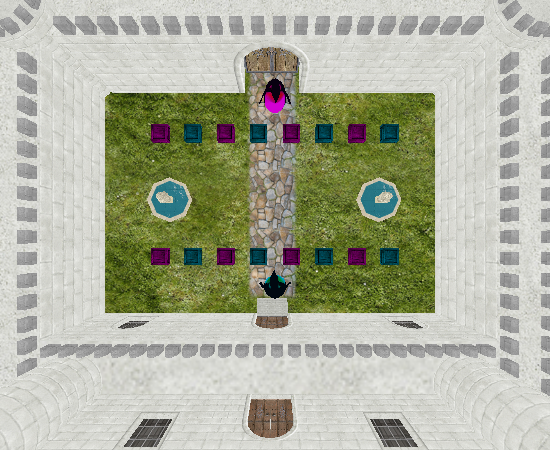
\includegraphics[width=6truecm, height=4truecm]{images/game.png}
	\caption{példakép a játékból}
\end{figure}

\Section{Az elemek vezérlése}

{\bf Billentyű, egér funkciók:}\\

Az ágens irányításához (lépés előre, hátra, fordulás, ugrás, doboz megfogása) különböző billenytűket haszbnáltam (például w,s,a,d) és a space-t billentyűket használtam fel, a  programból való kilépéshez az „ESC” billentyűt. Továbbá ez egér lehetővé teszi, hogy más szögből lássuk a jelenetet.


{ \bf A felhasznált függvények:}

\begin{itemize}
\item A \texttt{glutKeyBoardFunc()}-nek három paramétere van: \texttt{key} a generált ASCII karakter, az \texttt{x} és \texttt{y} pedig az egér pozíciója abban az időpontban, mikor a billentyű lenyomás történt a \texttt{GLUT} ablakhoz képest.

 Ezzel a funkcióval csak a kilépéshez szükséges \texttt{ESC} billentyű lenyomás kezelődött le és a \texttt{space}, a nyíl billentyűkhöz egy másik funkció szükséges.\cite{keyboardfunc}
\item A \texttt{glutSpecialFunc()} szükséges speciális billentyűk lenyomásának kezeléséhez,  
aminek szintén három paramétere van, a key, ami egy \texttt{GLUT\_KEY\_*} konstans, és az \texttt{x} és \texttt{y}, amik ugyanazt jelölik, mint az előző esetben, az egér relatív helyzetét az ablakhoz képest.\cite{keyboardspec}
\item A \texttt{glutMouseFunc()} az egér billentyűinek a lenyomását a  tudjuk nyomon követni, a mozgását pedig a \texttt{glutMotionFunc()}-al vagy a \texttt{glutPassiveMotionFunc()}-al. 

A glutMotionFunc azt az eshetőséget kezelei le, amikor egy vagy több billentyű lenyomás történt és közben lett mozgatva az egér. A \texttt{glutPassiveMotionFunc()} pedig azt, amikor úgy lett mozgatva az egér, hogy nem lett lenyomva egyetlen egér gomb sem.\cite{mousemot}\cite{mousefunc}
\end{itemize}
